\documentclass[11pt,a4paper]{article}

\usepackage[utf8]{inputenc}
\usepackage[T1]{fontenc}
\usepackage[spanish]{babel}
\usepackage{geometry}
\usepackage{graphicx}
\usepackage{array}
\usepackage{tabularx}
\usepackage{xcolor}
\usepackage{fancyhdr}
\usepackage{titlesec}
\usepackage{helvet}
\usepackage{ragged2e}
\usepackage{enumitem}
\usepackage{amsmath}
\usepackage{booktabs}
\usepackage{hyperref}

\renewcommand{\familydefault}{\sfdefault}
% babel-spanish names tables "Cuadro"; the report uses the Latin-American "Tabla".
\addto\captionsspanish{\renewcommand{\tablename}{Tabla}}
\graphicspath{{dist/}{./}}

\geometry{
  a4paper,
  left=3.0cm,
  right=3.0cm,
  top=2.35cm,
  bottom=2.35cm,
  headheight=1.9cm,
  headsep=0.45cm
}

\hypersetup{
  colorlinks=true,
  linkcolor=black,
  citecolor=black,
  urlcolor=blue
}

\setlength{\parindent}{0pt}
\setlength{\parskip}{0.22em}
\setlength{\tabcolsep}{6pt}
\renewcommand{\arraystretch}{1.08}

% Long unbreakable tokens (file names, inline math) otherwise overflow the margin.
\tolerance=1500
\emergencystretch=1.5em
\hyphenpenalty=200

\pagestyle{fancy}
\fancyhf{}
\fancyhead[L]{
\includegraphics[height=1.35cm]{reporte_tecnico_overleaf_logo.png}}
\fancyhead[R]{\vspace{0.1cm}\small FEIRNNR --- Carrera de Computaci\'on}
\renewcommand{\headrulewidth}{0.5pt}
\renewcommand{\footrulewidth}{0pt}
\makeatletter
\renewcommand{\headrule}{%
  {\color{gray!65}\hrule width\headwidth height\headrulewidth \vskip-\headrulewidth}%
}
\makeatother

\titleformat{\section}
  {\bfseries\fontsize{15}{17}\selectfont}
  {\thesection.}{0.8em}{}
\titlespacing*{\section}{0pt}{0.7ex}{0.2ex}

\titleformat{\subsection}
  {\bfseries\fontsize{12}{14}\selectfont}
  {\thesubsection}{0.7em}{}
\titlespacing*{\subsection}{0pt}{0.6ex}{0.15ex}

\newcolumntype{L}[1]{>{\RaggedRight\arraybackslash}p{#1}}
\newcolumntype{Y}{>{\RaggedRight\arraybackslash}X}
\newcolumntype{C}[1]{>{\centering\arraybackslash}p{#1}}

\begin{document}
\thispagestyle{fancy}

\vspace*{0.15cm}

\begin{center}
{\bfseries\fontsize{23}{26}\selectfont
Reporte T\'ecnico de Actividades\\
Pr\'actico-Experimentales Nro. 001\par}
\end{center}

\section{Datos de Identificaci\'on del Estudiante y la Pr\'actica}

\noindent
\begin{tabularx}{\textwidth}{|L{0.43\textwidth}|Y|}
\hline
\textbf{Nombre del estudiante} & Jaime Alejandro Land\'azuri Rom\'an \\ \hline
\textbf{Asignatura} & Simulaci\'on \\ \hline
\textbf{Ciclo} & 5 A \\ \hline
\textbf{Unidad} & U1: Introducci\'on a la Simulaci\'on \\ \hline
\textbf{Resultado de aprendizaje de la unidad} & R1. Aplica an\'alisis estad\'isticos de los
datos de la Simulaci\'on para mejorar la calidad de los resultados, bajo los principios de
solidaridad, transparencia, responsabilidad y honestidad. \\ \hline
\textbf{Pr\'actica Nro.} & 001 \\ \hline
\textbf{T\'itulo de la Pr\'actica} & Construcci\'on y simulaci\'on computacional de un
modelo matem\'atico \\ \hline
\textbf{Nombre del Docente} & Jos\'e O. Guam\'an Q. \\ \hline
\textbf{Fecha} & 01 de Octubre de 2026 / 02 de Octubre de 2026 \\ \hline
\textbf{Horario} & Jueves 10h30 -- 11h30 / Viernes 07h30 -- 09h30 \\ \hline
\textbf{Lugar} & Aula \\ \hline
\textbf{Tiempo planificado en el S\'ilabo} & 3 horas \\ \hline
\end{tabularx}

\section{Objetivo(s) de la Pr\'actica}

Comprender el proceso de construcci\'on de un modelo matem\'atico y analizar su
comportamiento mediante Python.

\begin{enumerate}[leftmargin=*]
  \item Identificar variables, par\'ametros y relaciones matem\'aticas de un sistema.
  \item Implementar un modelo matem\'atico en Python.
  \item Analizar gr\'aficamente la influencia de los par\'ametros.
\end{enumerate}

\section{Materiales y Reactivos}

\begin{itemize}[leftmargin=*]
  \item Computadora con m\'inimo 4\,GB de RAM y procesador de doble n\'ucleo o superior.
  \item Sistema operativo Linux o macOS.
  \item Python 3.10 o superior.
  \item NumPy y Matplotlib, seg\'un los materiales indicados por la gu\'ia.
  \item Editor de c\'odigo (Visual Studio Code, PyCharm o similar).
  \item Conexi\'on a Internet para instalar las herramientas.
\end{itemize}

La gu\'ia enumera \textbf{NumPy} y \textbf{Matplotlib} como materiales. En la
implementaci\'on efectivamente entregada, el \'unico paquete de terceros importado es
\texttt{matplotlib} (\texttt{views/graficas.py:5}); el c\'alculo de $H$, $N$, $Tf$ e $I$
es Python puro con aritm\'etica b\'asica y \texttt{round()}, por lo que NumPy no se
declara como dependencia. Se prefiere esta declaraci\'on honesta antes que instalar y
declarar librer\'ias sin uso.

\section{Fundamento Te\'orico}

Un modelo matem\'atico es una representaci\'on simplificada de un sistema real mediante
variables, par\'ametros y relaciones matem\'aticas, cuya finalidad es describir,
explicar o predecir el comportamiento del fen\'omeno bajo estudio
\cite{lawkelton2015,banks2010}. La construcci\'on del modelo implica decidir qu\'e
elementos del sistema se retienen (variables y relaciones) y qu\'e valores permanecen
fijos durante el an\'alisis (par\'ametros). En esta pr\'actica el sistema modelado es la
atm\'osfera durante una ventana de 24 horas, y la pregunta que el modelo responde es
\emph{en qu\'e horas existe posibilidad de lluvia} \cite{diaposSemana1}.

\subsection{Variables y par\'ametros}

Una \textbf{variable} es una magnitud cuyo valor cambia entre observaciones o a lo largo
del tiempo; un \textbf{par\'ametro} es una constante del modelo que se fija antes de
evaluarlo y no depende de la observaci\'on particular. En el modelo de esta pr\'actica:

\begin{itemize}[leftmargin=*]
  \item Son \textbf{variables} $H$ (humedad normalizada), $N$ (nubosidad normalizada) y
        $Tf$ (factor de temperatura): sus valores cambian hora a hora y provienen de las
        observaciones.
  \item Son \textbf{par\'ametros} $a$, $b$ y $c$: los coeficientes que ponderan cada
        variable en la combinaci\'on lineal. Permanecen constantes durante toda la corrida
        y definen la \emph{versi\'on} del modelo (original o ajustada).
\end{itemize}

\subsection{Normalizaci\'on de las variables}

La humedad y la nubosidad se registran como porcentajes, pero el \'indice se define sobre
el rango $[0,1]$; por eso ambas se normalizan dividiendo para 100:

\begin{equation}
H = \frac{\text{humedad }(\%)}{100},
\qquad
N = \frac{\text{nubosidad }(\%)}{100}
\label{eq:normalizacion}
\end{equation}

El factor de temperatura $Tf$ ya se expresa en el rango $[0,1]$ mediante la tabla de la
gu\'ia (tabla \ref{tab:tf}), que asigna un valor mayor a las temperaturas bajas porque
favorecen la condensaci\'on.

\begin{table}[htbp]
\centering
\caption{Factor de temperatura $Tf$ en funci\'on de la temperatura.}
\label{tab:tf}
\small
\begin{tabular}{cc}
\toprule
\textbf{Temperatura} & \textbf{$Tf$} \\
\midrule
$\leq 10$~°C & $1{,}00$ \\
$12$~°C      & $0{,}90$ \\
$14$~°C      & $0{,}80$ \\
$16$~°C      & $0{,}70$ \\
$18$~°C      & $0{,}60$ \\
$20$~°C      & $0{,}50$ \\
$22$~°C      & $0{,}40$ \\
$24$~°C      & $0{,}30$ \\
$26$~°C      & $0{,}20$ \\
$\geq 28$~°C & $0{,}10$ \\
\bottomrule
\end{tabular}
\end{table}

\subsection{\'Indice atmosf\'erico}

El modelo combina las tres variables normalizadas en una suma ponderada denominada
\emph{\'indice atmosf\'erico} $I$:

\begin{equation}
I = a\,H + b\,N + c\,Tf
\label{eq:indice}
\end{equation}

La gu\'ia propone los coeficientes originales $a = 0{,}50$, $b = 0{,}30$ y
$c = 0{,}20$, que suman $1{,}00$ y otorgan el mayor peso a la humedad. El \'indice queda
as\'i restringido al intervalo $[0,1]$, lo que permite interpretarlo como un indicador de
posibilidad de lluvia.

\subsection{Reglas de decisi\'on}

El valor de $I$ se traduce a un estado mediante los umbrales de la tabla \ref{tab:reglas}.
La lectura es acumulativa: cuanto m\'as alto el \'indice, mayor la posibilidad de lluvia.

\begin{table}[htbp]
\centering
\caption{Reglas de decisi\'on del modelo de lluvia.}
\label{tab:reglas}
\small
\begin{tabular}{lc}
\toprule
\textbf{\'Indice $I$} & \textbf{Estado} \\
\midrule
$I < 0{,}40$                  & Sin lluvia \\
$0{,}40 \leq I < 0{,}60$      & Baja posibilidad \\
$0{,}60 \leq I < 0{,}75$      & Lluvia probable \\
$I \geq 0{,}75$               & Lluvia \\
\bottomrule
\end{tabular}
\end{table}

\subsection{Ejemplo de la gu\'ia}

Con humedad $= 90$\,\%, nubosidad $= 80$\,\% y temperatura $= 18$~°C, la
normalizaci\'on \eqref{eq:normalizacion} y la tabla \ref{tab:tf} dan

\begin{equation}
H = 0{,}90, \qquad N = 0{,}80, \qquad Tf = 0{,}60
\end{equation}

y al aplicar la ecuaci\'on \eqref{eq:indice} con los coeficientes originales:

\begin{equation}
I = 0{,}50\,(0{,}90) + 0{,}30\,(0{,}80) + 0{,}20\,(0{,}60) = 0{,}81
\label{eq:ejemplo}
\end{equation}

Como $I = 0{,}81 \geq 0{,}75$, el modelo clasifica el estado como \textbf{Lluvia}. Este
c\'alculo reproduce exactamente el ejemplo de la gu\'ia y se us\'o como caso de
verificaci\'on del programa.

\section{Procedimiento / Metodolog\'ia Ejecutada}

El desarrollo sigui\'o las etapas indicadas por la gu\'ia de actividades
pr\'actico-experimentales Nro. 001 \cite{guaman2026ape1}.

\subsection{Preparaci\'on del entorno}

Se trabaj\'o con Python 3.10 o superior dentro de un entorno virtual para aislar las
dependencias del proyecto:

\begin{itemize}[leftmargin=*]
  \item Creaci\'on del entorno: \texttt{python -m venv venv} y activaci\'on del
        mismo con
        \texttt{source venv/bin/activate}.
  \item Instalaci\'on de dependencias: \texttt{pip install -r requirements.txt}, donde
        \texttt{requirements.txt} declara \texttt{matplotlib>=3.7}.
  \item Ejecuci\'on del programa desde el directorio \texttt{APE1} mediante
        \texttt{python -m views.main}.
\end{itemize}

\subsection{Datos horarios de entrada}

Se utilizaron las nueve observaciones horarias definidas por la gu\'ia, declaradas en
\texttt{models/datasets.py} como la constante \texttt{DATOS\_HORARIOS} (tabla
\ref{tab:datos}). Cada registro contiene hora, humedad, nubosidad y temperatura.

\begin{table}[htbp]
\centering
\caption{Observaciones horarias de entrada (gu\'ia Nro. 001).}
\label{tab:datos}
\small
\begin{tabular}{cccc}
\toprule
\textbf{Hora} & \textbf{Humedad (\%)} & \textbf{Nubosidad (\%)} & \textbf{Temperatura (°C)} \\
\midrule
06:00 & 65 & 40 & 14 \\
08:00 & 70 & 50 & 16 \\
10:00 & 68 & 45 & 18 \\
12:00 & 60 & 30 & 22 \\
14:00 & 75 & 70 & 20 \\
16:00 & 85 & 85 & 18 \\
18:00 & 92 & 95 & 16 \\
20:00 & 88 & 90 & 17 \\
22:00 & 80 & 75 & 15 \\
\bottomrule
\end{tabular}
\end{table}

\subsection{Implementaci\'on del modelo}

El c\'odigo se organiz\'o en tres capas (modelo, controlador y vista) con la siguiente
responsabilidad por archivo:

\begin{itemize}[leftmargin=*]
  \item \texttt{models/datasets.py}: contiene la tabla del factor de temperatura
        (\texttt{tabla\_tf}), los coeficientes del modelo original
        (\texttt{COEFICIENTES\_ORIGINAL} $= \{0{,}50,\,0{,}30,\,0{,}20\}$) y del modelo
        ajustado (\texttt{COEFICIENTES\_AJUSTADO} $= \{0{,}40,\,0{,}35,\,0{,}25\}$), los
        datos horarios \texttt{DATOS\_HORARIOS} y las reglas \texttt{REGLAS\_LLUVIA}.
  \item \texttt{controller/utils.py}: implementa la funci\'on \texttt{tf\_dict}, que
        redondea la temperatura al m\'ultiplo de $2$~°C m\'as cercano con
        \texttt{round(temp / 2) * 2} y limita el resultado a los extremos de la tabla
        ($\leq 10$~°C $\rightarrow 1{,}00$; $\geq 28$~°C $\rightarrow 0{,}10$); la
        funci\'on \texttt{indice}, que eval\'ua la ecuaci\'on \eqref{eq:indice}; y la
        funci\'on \texttt{clasificar}, que aplica las reglas de la tabla \ref{tab:reglas}.
  \item \texttt{controller/tabla.py}: construye la tabla horaria completa con
        \texttt{construir\_tabla} (calcula $H$, $N$, $Tf$, $I$ y el estado de cada hora) y
        la imprime con \texttt{imprimir\_tabla}.
  \item \texttt{views/graficas.py}: genera las cuatro figuras de la pr\'actica
        (\texttt{indice\_original.png}, \texttt{indice\_ajustado.png},
        \texttt{indice\_comparacion.png} y \texttt{variables\_hora.png}) y las guarda en
        \texttt{dist/}.
  \item \texttt{views/main.py}: punto de entrada por consola; construye e imprime la
        tabla del modelo original y la del ajustado, genera las gr\'aficas y, con la
        bandera \texttt{-{}-interactivo}, solicita humedad, nubosidad y temperatura para
        clasificar una consulta puntual.
\end{itemize}

\subsection{Generaci\'on de resultados}

Se ejecut\'o \texttt{python -m views.main} para producir la tabla horaria de ambos
modelos y las cuatro figuras. Con el fin de verificar el caso de la gu\'ia se comprob\'o
manualmente el ejemplo de la ecuaci\'on \eqref{eq:ejemplo}, que arroja $I = 0{,}81$ y el
estado \emph{Lluvia}. Los valores que se presentan en la secci\'on \ref{sec:resultados}
provienen de esta corrida reproducible del programa.

\section{Resultados}
\label{sec:resultados}

\subsection{Modelo original ($I = 0{,}50H + 0{,}30N + 0{,}20Tf$)}

La tabla \ref{tab:original} presenta la tabla horaria del modelo original con los valores
calculados por el programa, y la figura \ref{fig:original} su representaci\'on gr\'afica.
El caso 06:00 arroja $I = 0{,}6050$ (estado \emph{Lluvia probable}) y el caso 18:00
$I = 0{,}8850$ (estado \emph{Lluvia}), valores que coinciden con la verificaci\'on
esperada.

\begin{table}[htbp]
\centering
\caption{Tabla horaria del modelo original. Valores calculados por
\texttt{controller/tabla.py}.}
\label{tab:original}
\small
\setlength{\tabcolsep}{4pt}
\begin{tabular}{L{1.2cm} C{1.7cm} C{1.9cm} C{1.0cm} C{0.8cm} C{0.8cm} C{0.8cm} C{1.2cm} L{2.6cm}}
\toprule
{\footnotesize\textbf{Hora}} & {\footnotesize\textbf{Humedad}} &
{\footnotesize\textbf{Nubosidad}} & {\footnotesize\textbf{Temp.}} &
{\footnotesize\textbf{$H$}} & {\footnotesize\textbf{$N$}} &
{\footnotesize\textbf{$Tf$}} & {\footnotesize\textbf{\'Indice}} &
{\footnotesize\textbf{Estado}} \\
\midrule
06:00 & 65 & 40 & 14 & 0{,}65 & 0{,}40 & 0{,}80 & 0{,}6050 & Lluvia probable \\
08:00 & 70 & 50 & 16 & 0{,}70 & 0{,}50 & 0{,}70 & 0{,}6400 & Lluvia probable \\
10:00 & 68 & 45 & 18 & 0{,}68 & 0{,}45 & 0{,}60 & 0{,}5950 & Baja posibilidad \\
12:00 & 60 & 30 & 22 & 0{,}60 & 0{,}30 & 0{,}40 & 0{,}4700 & Baja posibilidad \\
14:00 & 75 & 70 & 20 & 0{,}75 & 0{,}70 & 0{,}50 & 0{,}6850 & Lluvia probable \\
16:00 & 85 & 85 & 18 & 0{,}85 & 0{,}85 & 0{,}60 & 0{,}8000 & Lluvia \\
18:00 & 92 & 95 & 16 & 0{,}92 & 0{,}95 & 0{,}70 & 0{,}8850 & Lluvia \\
20:00 & 88 & 90 & 17 & 0{,}88 & 0{,}90 & 0{,}70 & 0{,}8500 & Lluvia \\
22:00 & 80 & 75 & 15 & 0{,}80 & 0{,}75 & 0{,}70 & 0{,}7650 & Lluvia \\
\bottomrule
\end{tabular}
\end{table}

\begin{figure}[htbp]
\centering
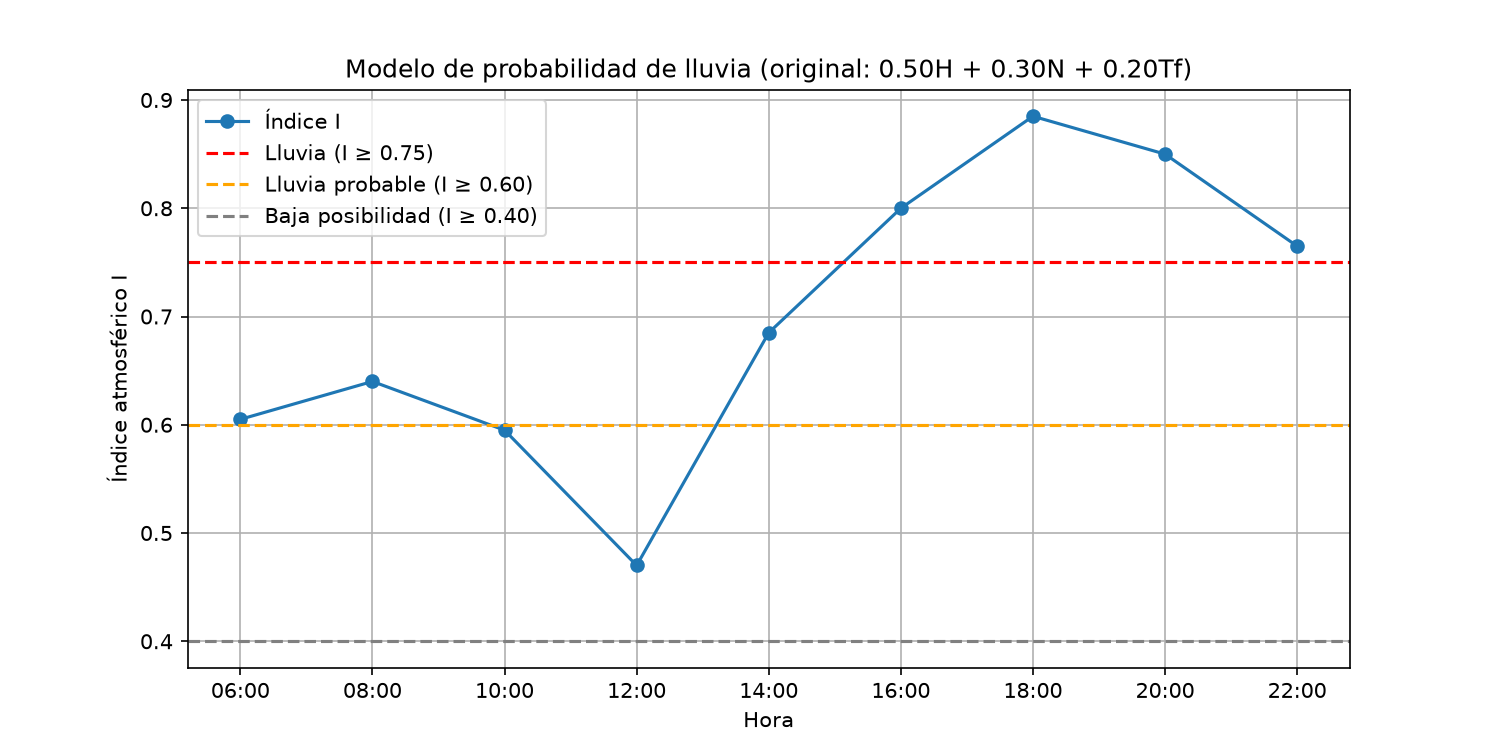
\includegraphics[width=0.92\textwidth]{indice_original.png}
\caption{\'Indice atmosf\'erico por hora del modelo original
($0{,}50H + 0{,}30N + 0{,}20Tf$). Las l\'ineas discontinuas marcan los umbrales de
decisi\'on $0{,}40$, $0{,}60$ y $0{,}75$; los puntos por encima de la l\'inea roja
corresponden a las horas con estado \emph{Lluvia}.}
\label{fig:original}
\end{figure}

\subsection{Modelo ajustado ($I = 0{,}40H + 0{,}35N + 0{,}25Tf$)}

La gu\'ia pide \emph{ajustar el modelo y llenar de nuevo la misma tabla}. Se eligi\'o un
nuevo juego de coeficientes que tambi\'en suma $1{,}00$, reduciendo el peso de la humedad
y aumentando el de la nubosidad y el factor de temperatura. La tabla \ref{tab:ajustado}
contiene el resultado y la figura \ref{fig:ajustado} su gr\'afica.

\begin{table}[htbp]
\centering
\caption{Tabla horaria del modelo ajustado. Valores calculados por
\texttt{controller/tabla.py}.}
\label{tab:ajustado}
\small
\setlength{\tabcolsep}{4pt}
\begin{tabular}{L{1.2cm} C{1.7cm} C{1.9cm} C{1.0cm} C{0.8cm} C{0.8cm} C{0.8cm} C{1.2cm} L{2.6cm}}
\toprule
{\footnotesize\textbf{Hora}} & {\footnotesize\textbf{Humedad}} &
{\footnotesize\textbf{Nubosidad}} & {\footnotesize\textbf{Temp.}} &
{\footnotesize\textbf{$H$}} & {\footnotesize\textbf{$N$}} &
{\footnotesize\textbf{$Tf$}} & {\footnotesize\textbf{\'Indice}} &
{\footnotesize\textbf{Estado}} \\
\midrule
06:00 & 65 & 40 & 14 & 0{,}65 & 0{,}40 & 0{,}80 & 0{,}6000 & Lluvia probable \\
08:00 & 70 & 50 & 16 & 0{,}70 & 0{,}50 & 0{,}70 & 0{,}6300 & Lluvia probable \\
10:00 & 68 & 45 & 18 & 0{,}68 & 0{,}45 & 0{,}60 & 0{,}5795 & Baja posibilidad \\
12:00 & 60 & 30 & 22 & 0{,}60 & 0{,}30 & 0{,}40 & 0{,}4450 & Baja posibilidad \\
14:00 & 75 & 70 & 20 & 0{,}75 & 0{,}70 & 0{,}50 & 0{,}6700 & Lluvia probable \\
16:00 & 85 & 85 & 18 & 0{,}85 & 0{,}85 & 0{,}60 & 0{,}7875 & Lluvia \\
18:00 & 92 & 95 & 16 & 0{,}92 & 0{,}95 & 0{,}70 & 0{,}8755 & Lluvia \\
20:00 & 88 & 90 & 17 & 0{,}88 & 0{,}90 & 0{,}70 & 0{,}8420 & Lluvia \\
22:00 & 80 & 75 & 15 & 0{,}80 & 0{,}75 & 0{,}70 & 0{,}7575 & Lluvia \\
\bottomrule
\end{tabular}
\end{table}

\begin{figure}[htbp]
\centering
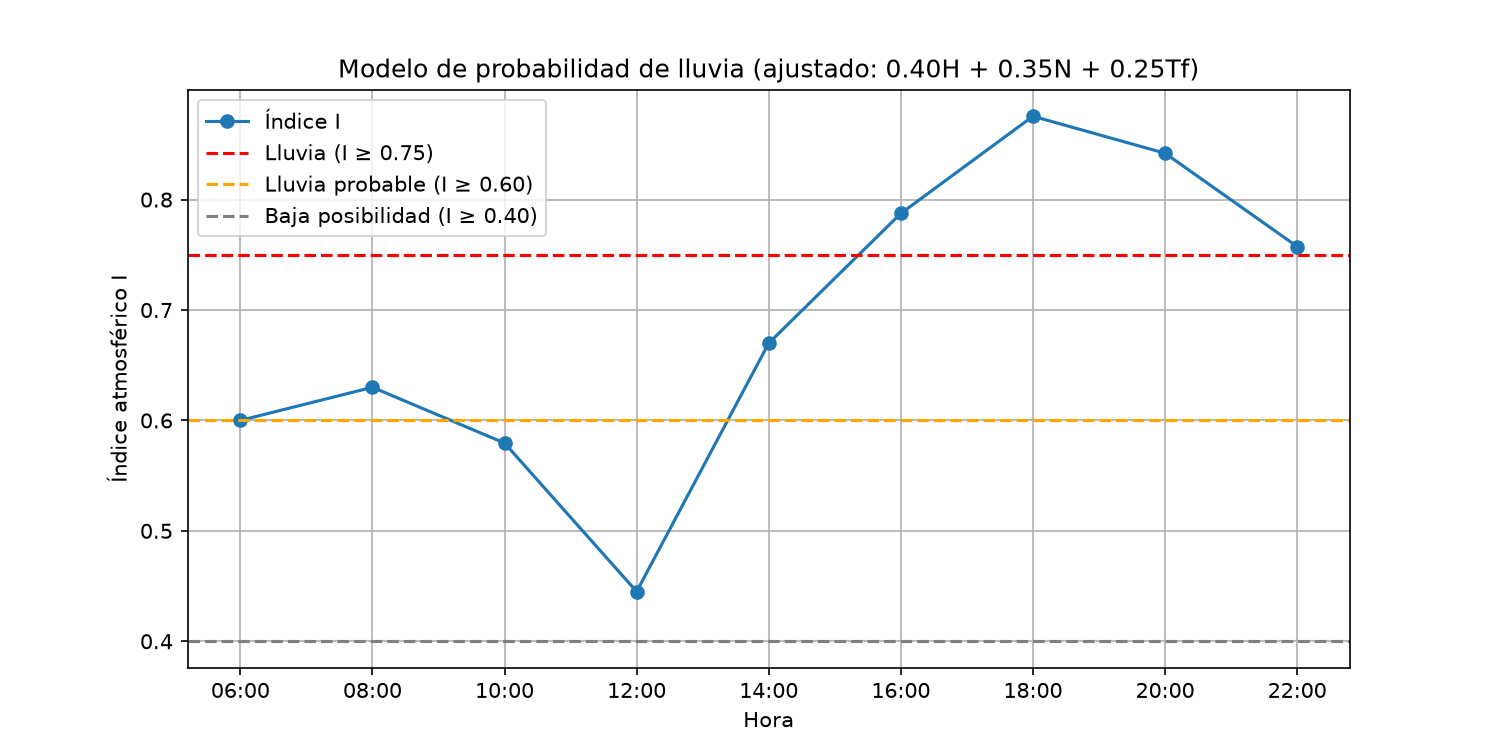
\includegraphics[width=0.92\textwidth]{indice_ajustado.png}
\caption{\'Indice atmosf\'erico por hora del modelo ajustado
($0{,}40H + 0{,}35N + 0{,}25Tf$) con los mismos umbrales de decisi\'on. La forma de la
curva es id\'entica a la del modelo original, pero desplazada hacia abajo en todos los
puntos.}
\label{fig:ajustado}
\end{figure}

\subsection{Comparaci\'on de ambos modelos}

La figura \ref{fig:comparacion} superpone las dos series. La figura
\ref{fig:variables} muestra, por separado, la evoluci\'on de las variables normalizadas
$H$, $N$ y $Tf$ que alimentan al modelo.

\begin{figure}[htbp]
\centering
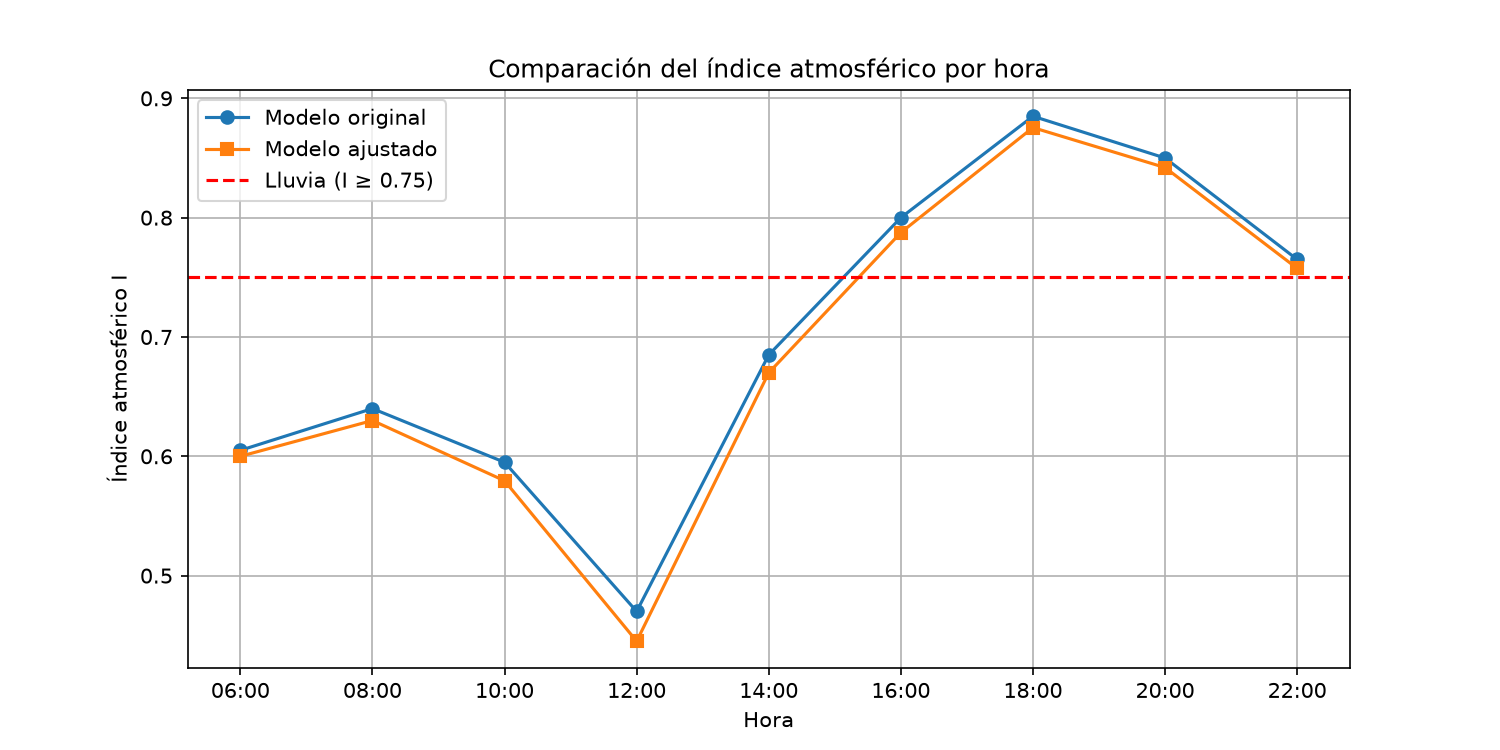
\includegraphics[width=0.92\textwidth]{indice_comparacion.png}
\caption{Comparaci\'on del \'indice por hora entre el modelo original y el ajustado. Las
dos curvas conservan el mismo perfil y la misma clasificaci\'on; el modelo ajustado queda
por debajo porque reparte el peso hacia $N$ y $Tf$. La l\'inea roja marca el umbral de
\emph{Lluvia} ($I \geq 0{,}75$).}
\label{fig:comparacion}
\end{figure}

\begin{figure}[htbp]
\centering
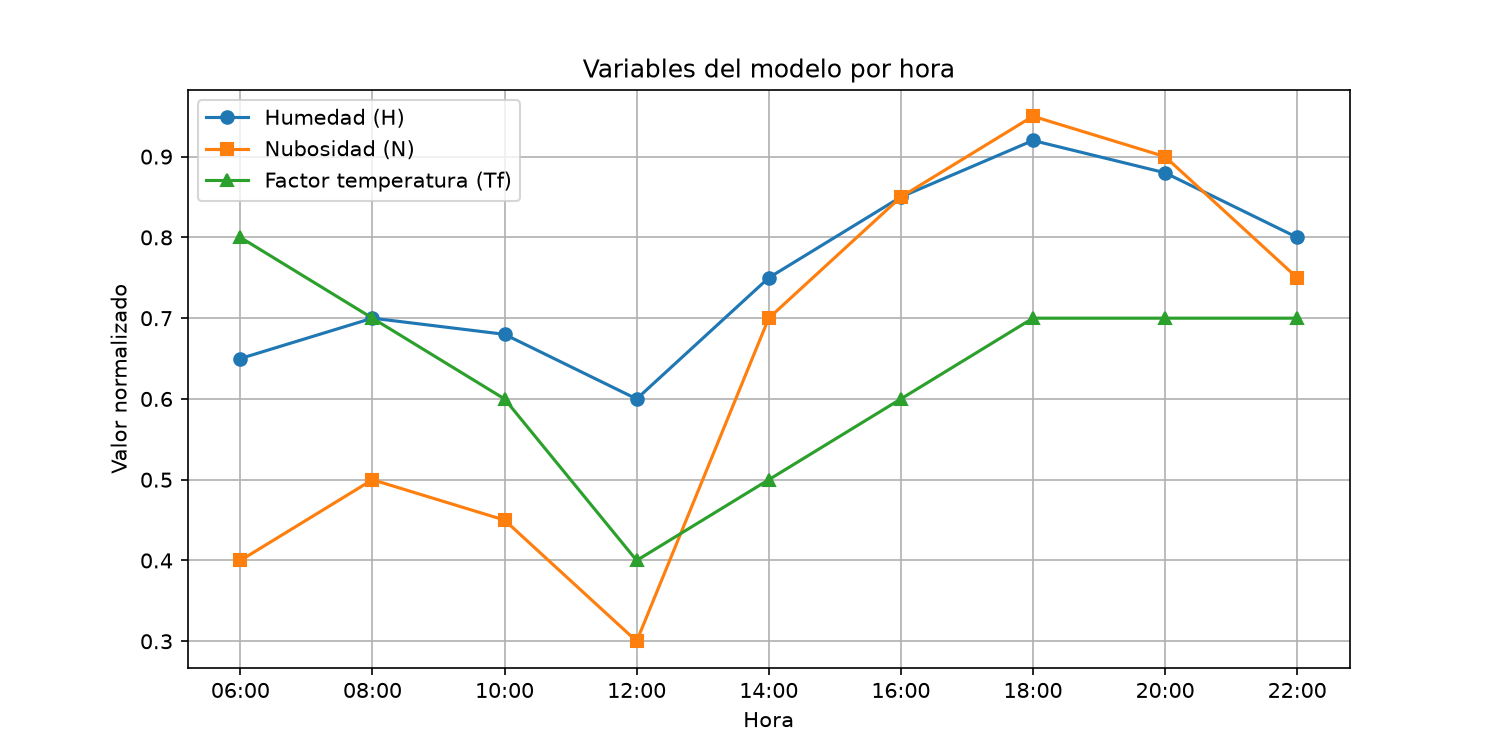
\includegraphics[width=0.92\textwidth]{variables_hora.png}
\caption{Evoluci\'on horaria de las variables del modelo: humedad normalizada $H$,
nubosidad normalizada $N$ y factor de temperatura $Tf$. $H$ y $N$ crecen hacia el final
del d\'ia (m\'as humedad y nubes), mientras $Tf$ se mantiene alto en las horas fr\'ias.}
\label{fig:variables}
\end{figure}

\subsection{Lectura de los estados}

En ambos modelos las reglas de la tabla \ref{tab:reglas} producen la misma
clasificaci\'on, porque los umbrales son bandas anchas y las diferencias entre los dos
\'indices son pequeñas:

\begin{itemize}[leftmargin=*]
  \item \textbf{Lluvia} ($I \geq 0{,}75$): 16:00, 18:00, 20:00 y 22:00.
  \item \textbf{Lluvia probable} ($0{,}60 \leq I < 0{,}75$): 06:00, 08:00 y 14:00.
  \item \textbf{Baja posibilidad} ($0{,}40 \leq I < 0{,}60$): 10:00 y 12:00.
  \item \textbf{Sin lluvia} ($I < 0{,}40$): ninguna hora.
\end{itemize}

\section{Interpretaci\'on Matem\'atica del Comportamiento}

\begin{itemize}[leftmargin=*]
  \item \textbf{Sensibilidad a los coeficientes.} Cambiar los coeficientes desplaza el
        \'indice sin alterar la forma de la serie. La diferencia entre el modelo ajustado y
        el original es $\Delta I = -0{,}10\,H + 0{,}05\,N + 0{,}05\,Tf
        = 0{,}05\,(N + Tf - 2H)$. Por ejemplo, 06:00 pasa de $0{,}6050$ a $0{,}6000$
        ($-0{,}0050$), 10:00 de $0{,}5950$ a $0{,}5795$ ($-0{,}0155$) y 16:00 de
        $0{,}8000$ a $0{,}7875$ ($-0{,}0125$).
  \item \textbf{Reparto del peso.} El modelo ajustado otorga m\'as peso a $N$ y $Tf$ y
        menos a $H$. Como en estas observaciones $H$ es la variable normalizada m\'as
        grande, el t\'ermino $-0{,}10\,H$ domina y el \'indice baja en \emph{todas} las
        horas; la mayor reducci\'on ocurre a las 12:00 ($-0{,}0250$) y la menor a las
        06:00 ($-0{,}0050$). Si $N + Tf > 2H$ el ajuste subir\'ia el \'indice, lo que
        confirma que el efecto depende de la relaci\'on entre las variables y no de un
        signo fijo.
  \item \textbf{Los umbrales operan sobre el mismo rango.} Como los coeficientes de cada
        versi\'on suman $1{,}00$ y las tres variables est\'an en $[0,1]$, el \'indice
        siempre pertenece a $[0,1]$. Por eso los umbrales $0{,}40$, $0{,}60$ y $0{,}75$
        son comparables entre modelos y la clasificaci\'on no se distorsiona al cambiar
        los coeficientes.
  \item \textbf{Estabilidad de la clasificaci\'on.} Aunque los valores de $I$ cambian
        entre versiones, los estados son los mismos en este conjunto de datos porque
        ninguna diferencia cruza un umbral. El caso m\'as ajustado es 22:00, cuyo
        \'indice baja de $0{,}7650$ a $0{,}7575$ y permanece apenas por encima de
        $0{,}75$: una variaci\'on adicional de los coeficientes podr\'ia cambiar ese
        estado.
  \item \textbf{Modelo determin\'istico.} El \'indice es una funci\'on expl\'icita de las
        observaciones: para una misma hora, humedad, nubosidad y temperatura, el
        resultado es siempre el mismo. No hay aleatoriedad ni realimentaci\'on entre
        horas, de modo que cada fila se calcula de forma independiente y el modelo es
        reproducible por construcci\'on.
\end{itemize}

\section{Preguntas de Control}

\begin{enumerate}[leftmargin=*]

  \item \textbf{¿Qu\'e es un modelo matem\'atico?}

  Es una representaci\'on simplificada de un sistema o fen\'omeno real mediante
  variables, par\'ametros y relaciones matem\'aticas (ecuaciones, funciones y reglas),
  construida para describir, explicar o predecir su comportamiento
  \cite{lawkelton2015,banks2010}. Un modelo no reproduce el sistema en todos sus
  detalles: selecciona los elementos relevantes para la pregunta que se desea responder.
  En esta pr\'actica, el modelo es el \'indice $I = aH + bN + cTf$ junto con las reglas
  de decisi\'on que lo traducen a estados de lluvia.

  \item \textbf{¿Cu\'al es la diferencia entre variable y par\'ametro?}

  Una \textbf{variable} cambia entre observaciones o con el tiempo y su valor se toma de
  los datos; un \textbf{par\'ametro} es una constante que se fija antes de evaluar el
  modelo y permanece igual durante toda la corrida. En este modelo, $H$, $N$ y $Tf$ son
  variables porque cambian hora a hora seg\'un las observaciones, mientras $a$, $b$ y $c$
  son par\'ametros: los coeficientes $0{,}50$, $0{,}30$ y $0{,}20$ del modelo original
  (o $0{,}40$, $0{,}35$ y $0{,}25$ del ajustado) definen la versi\'on del modelo y no
  dependen de la hora.

  \item \textbf{¿Qu\'e representa $P_0$?}

  $P_0$ es la \emph{poblaci\'on inicial}, es decir, el valor de la poblaci\'on en el
  instante $t = 0$. En la soluci\'on $P(t) = P_0\,e^{rt}$ act\'ua como la condici\'on
  inicial que selecciona una \'unica curva dentro de la familia de soluciones: cambiando
  $P_0$ cambia la escala de toda la trayectoria, pero no su forma exponencial.

  \item \textbf{¿Qu\'e ocurre cuando $r < 0$?}

  Si la tasa de crecimiento es negativa, la poblaci\'on decrece exponencialmente:
  $P(t) = P_0\,e^{rt}$ disminuye de forma asint\'otica hacia $0$ sin alcanzarlo en tiempo
  finito. El sistema presenta realimentaci\'on negativa, pues cada vez hay menos
  individuos que aporten nuevos nacimientos.

  \item \textbf{¿Qu\'e limitaciones tiene el modelo exponencial?}

  Su principal limitaci\'on es que supone recursos ilimitados: al no incluir una capacidad
  de carga, la poblaci\'on crece sin cota para $r > 0$, lo que solo es v\'alido en la fase
  inicial. Tampoco contempla la competencia por recursos, la saturaci\'on del medio ni
  retardos o factores externos, y no admite cambios de r\'egimen; para corregirlo se
  requiere un modelo log\'istico o de otro tipo que acote el crecimiento.

\end{enumerate}

\textbf{Nota.} Las preguntas 3, 4 y 5 ($P_0$, $r < 0$ y el modelo exponencial)
corresponden a la plantilla de \textbf{crecimiento poblacional} de la pr\'actica APE 002 y
\textbf{no} describen el modelo de \'indice atmosf\'erico de esta pr\'actica. Se responden
arriba en sus propios t\'erminos porque aparecen en la gu\'ia, pero sus conceptos no se
aplican al modelo $I = aH + bN + cTf$ desarrollado en este reporte.

\section{Conclusiones}

\begin{itemize}[leftmargin=*]
  \item Se implement\'o y verific\'o el modelo de \'indice atmosf\'erico
        $I = aH + bN + cTf$ ejecutando el programa
        (\texttt{python -m views.main}), que reproduce el ejemplo de la gu\'ia
        ($I = 0{,}81 \rightarrow$ \emph{Lluvia}) y genera las tablas horarias de ambos
        modelos.

  \item Tanto la versi\'on original como la ajustada llenan la tabla completa de las
        nueve horas y producen sus gr\'aficas: \texttt{indice\_original.png},
        \texttt{indice\_ajustado.png}, \texttt{indice\_comparacion.png} y
        \texttt{variables\_hora.png}, guardadas en \texttt{dist/}.

  \item Las horas de lluvia coinciden entre los dos modelos (16:00, 18:00, 20:00 y
        22:00), con \emph{Lluvia probable} a las 06:00, 08:00 y 14:00 y \emph{Baja
        posibilidad} a las 10:00 y 12:00; ninguna hora queda sin lluvia.

  \item El ajuste de coeficientes modifica el valor de $I$ en todas las horas
        (por ejemplo, 06:00 de $0{,}6050$ a $0{,}6000$ y 16:00 de $0{,}8000$ a
        $0{,}7875$), pero \textbf{no cambia los estados} en este conjunto de datos,
        porque las diferencias no cruzan ning\'un umbral; el caso m\'as cercano al l\'imite
        es 22:00, con $0{,}7575$ frente al umbral $0{,}75$.

  \item El modelo es \textbf{determin\'istico} y reproducible: cada fila se calcula de
        forma independiente a partir de las observaciones, sin aleatoriedad. La gu\'ia
        solicitaba adem\'as una implementaci\'on en Java; esta entrega incluye
        \'unicamente la versi\'on en Python.
\end{itemize}

\newpage

\section{Declaraci\'on de Uso de Inteligencia Artificial}

En cumplimiento de los principios de solidaridad, transparencia, responsabilidad y
honestidad establecidos en el resultado de aprendizaje R1, se declara lo siguiente:

\begin{enumerate}[leftmargin=*]
  \item \textbf{Porcentaje de uso.} Se emplearon herramientas de inteligencia artificial
        como apoyo acotado, estimado en \textbf{no m\'as del 20\%} del trabajo total de
        la pr\'actica.

  \item \textbf{El razonamiento del estudiante no fue reemplazado.} La comprensi\'on del
        problema atmosf\'erico, la interpretaci\'on del modelo
        $I = 0{,}50H + 0{,}30N + 0{,}20Tf$, la elecci\'on de los coeficientes del modelo
        ajustado y la clasificaci\'on seg\'un las reglas de la gu\'ia fueron razonadas,
        revisadas y validadas por el estudiante.

  \item \textbf{Alcance del apoyo recibido.} El uso de la IA se limit\'o a tareas
        auxiliares: la redacci\'on del c\'odigo Python a partir de las ecuaciones y la
        tabla de la gu\'ia, el formato de las gr\'aficas y la revisi\'on de estilo y
        redacci\'on de la documentaci\'on. Ninguna decisi\'on metodol\'ogica se deleg\'o a
        la herramienta.

  \item \textbf{Verificaci\'on de resultados.} Todos los valores presentados en este
        reporte provienen de la ejecuci\'on reproducible del programa desarrollado
        (\texttt{python -m views.main}). El estudiante ejecut\'o, comprob\'o y
        comprendi\'o cada resultado antes de incluirlo.

  \item \textbf{Responsabilidad.} El estudiante asume la responsabilidad total sobre el
        contenido, la exactitud, la originalidad y las conclusiones del trabajo entregado.
\end{enumerate}

\bibliographystyle{IEEEtran}
\bibliography{referencias}

\end{document}
